\chapter{System Implementation}\label{cha:Implementation}
In this chapter, we will talk about the implementation datail of the proposed system and will focus on the function on data service server's environment and techeniques.

\section{Data Service Server Environment}

\subsection{Node.js}
Node.js \cite{nodejs} is a open sourse JavaScript application framework written in C \cite{clang}, C++ \cite{cplus} and JavaScript \cite{javascript}
Node.js can run on many operation systems like Microsoft Windows, Linux, Mac and embedded system like Raspberry, Cubieboard.
There are many advantages of Node.js.
To begin with, it use V8 JavaScript engine to boost performance, which make it much more better than other script language.
Second, it's event driven and non-blocking I/O feature is surprisingly appropriate to both front-end and back-end of web application.
Third, as a popular programming language like Python and Ruby, there are many third-party module on the word wild web that developers around the world wrote,
we can make use of these modules to accelerate time developing apps. Whats more, the module is managed properly by nodejs package management (npm), which make it easy to import modules.
\subsection{Asynchronous Process Control}
Since Node.js is JaveScript with extensional function, the event-driven feature in JaveScript is to Node.js, as a result we can often see asynchronous design model in JavaScript code.
The idea of event-driven and asynchronous is run the job need long time to finish in the back-end event engine to avoid the job block all the process.
After that, we will set a callback function to inform the process when the time-comsuming job is done.
Figure \ref{fig:asynchornous} shows the idea of asynchronous process control.

\begin{figure}[H]
    \centering
    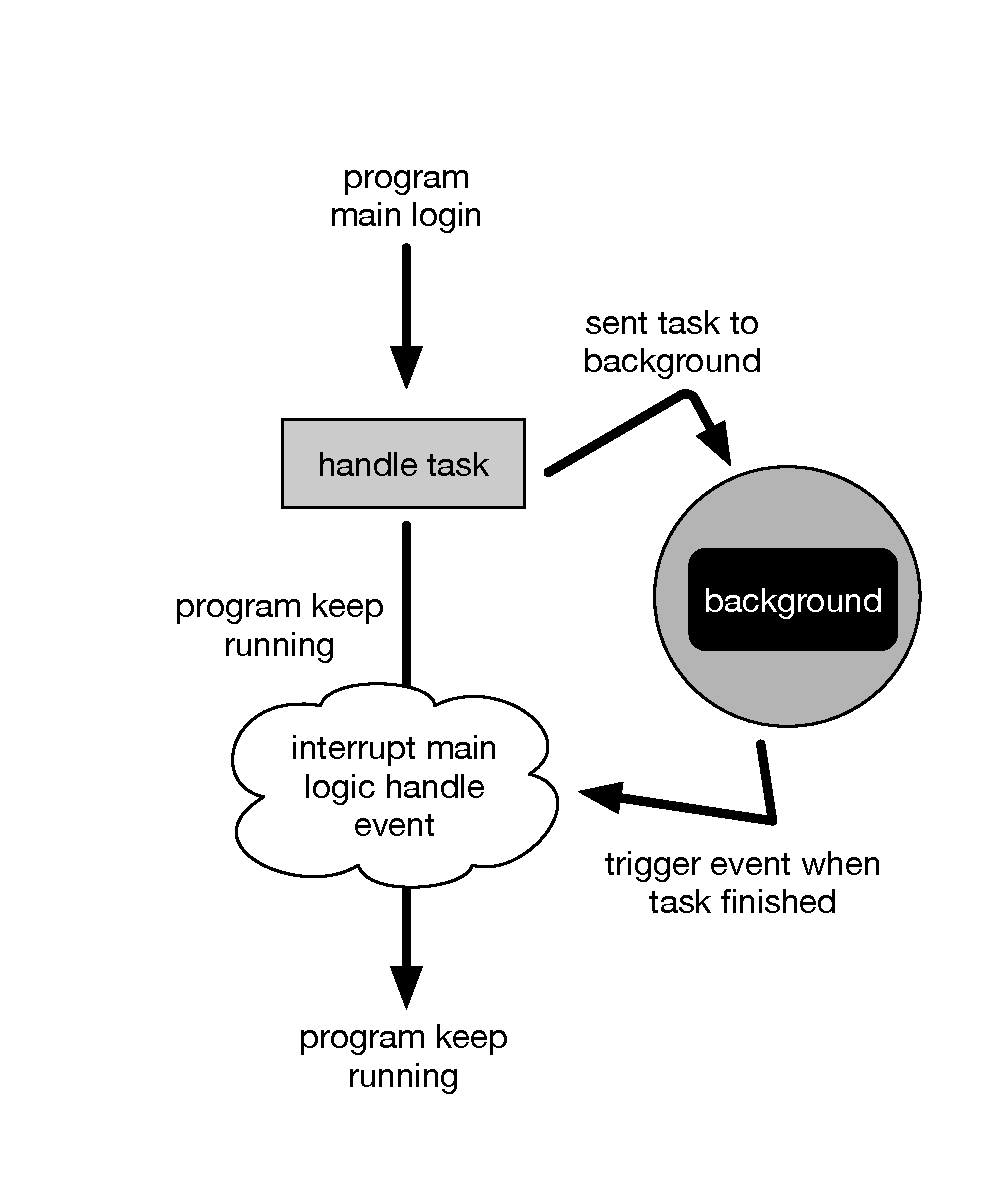
\includegraphics[width = 0.8\textwidth]{fig/asynchonous-process.eps}
    \caption{Asynchorous process control model}
    \label{fig:asynchornous}
\end{figure}


\subsection{MongoDB}
MongoDB \cite{mongodb} is an free and open source nosql database, data in mongodb saved as a json-like document with dynamic schemas (BSON).
MongoDB can handle big data in scale in Terabytes with its high performance and it's tableless database structure also make it easy to integrate data in certain type of applications eaiser and faster.

\subsection{Google Cloud Platform}
Google Cloud Platform \cite{googlecloud} is a platform integrates Iaas, Paas and Saas.
According to the website, it provides eight categories of service, including basic virtual machine renting, database hosting, big data analysis, machine learning and more.

\subsection{Iron Worker}
Ironworker \cite{ironworker} is a service on Iron.io, which make developer setup a worker on website with flexible scheduling setting.
Once developer setup the worker, Ironworker will monitor the worker, and if any thing go wrong, Ironworker will notify you by email with detail information.

\section{Server Setup}
In order to construct out server, we rent a VM instance machine type:n1-standard-4 (4 vCPUs, 15 GB memory), and on top of that we run a mongoDB on the same machine.
After setting up the environment, we execute the nodejs api server conneted with the mongoDB to save the data to database and to provide other API for query data.
Among APIs the server provide, there is a API will triggered by the worker we set onece a day, this API is designed for execute a python script, which is our data analysis system that will update the refine data (see Figure \ref{fig:serversetup}).
\begin{figure}[H]
    \centering
    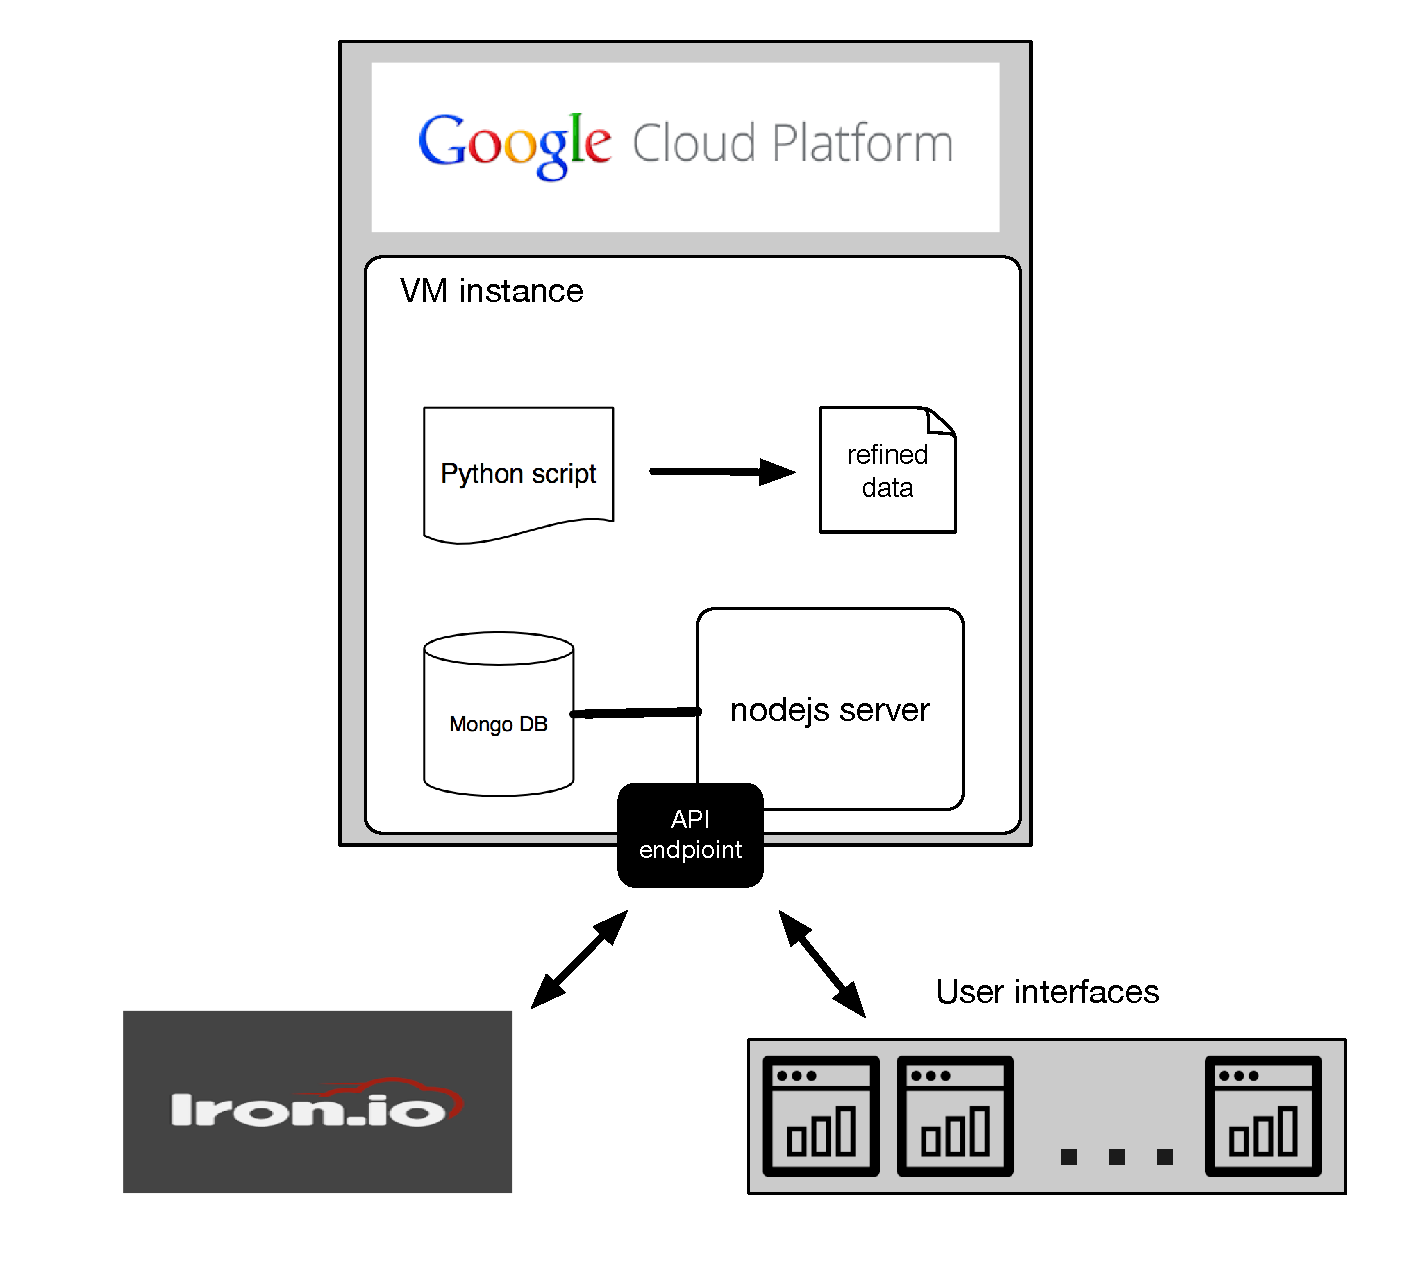
\includegraphics[width = 0.8\textwidth]{fig/serversetup.eps}
    \caption{server setup}
    \label{fig:serversetup}
\end{figure}

\section{API Server}
\section{Analysis System}
